\documentclass{article}
\usepackage[utf8]{inputenc}
\usepackage[danish,english]{babel}
\usepackage{alphabeta} 
\usepackage{
    amsmath, % \begin{align}
    amssymb, % math symbols såsom \rightarrow 
    wrapfig, % indsæt figurer ved siden af tekst
    float, % vælge placering af figures med [H]
    enumitem, % ændre label på enumeration
    fancyhdr, % header og footer
    xcolor, % tekstfarve mm.
    colortbl, % farve tabellers celler
    tabularx, % mere kontrol over tabeller
    listings, % kodebokse
    hyperref, % embed links
    nameref, % referere til mere end bare label-number
    multirow, % multiple row in tables
}
\usepackage{hyperref}

\hypersetup{
    colorlinks=true,
    linkcolor=blue,
    filecolor=magenta,      
    urlcolor=cyan
}

\usepackage{tabularx}
\usepackage[pdftex]{graphicx}
\graphicspath{ {images/} }
\usepackage[top=1in, bottom=1in, left=1in, right=1in]{geometry}
\linespread{1.3} % This is one and a half linespread
\setlength{\parskip}{8pt plus2pt minus2pt}
\usepackage{xparse}
\usepackage{csquotes}
\usepackage{biblatex}
\addbibresource{references.bib}

\pagestyle{fancy}
\fancyhead[LR]{} 
\renewcommand{\headrulewidth}{0pt} 
\renewcommand{\footrulewidth}{0pt} 

\widowpenalty 10000
\clubpenalty 10000

\newcommand{\eat}[1]{}
\newcommand{\HRule}{\rule{\linewidth}{0.5mm}}
\renewcommand{\arraystretch}{1.5}

\usepackage[official]{eurosym}
\usepackage{pdfpages}
\usepackage{enumitem}
\setlist{nolistsep,noitemsep}
\usepackage{lipsum}

\usepackage{fancyhdr,xcolor}

\let\oldheadrule\headrule% Copy \headrule into \oldheadrule
\renewcommand{\headrule}{\color{red}\oldheadrule}% Add colour to \headrule

\setlength{\parindent}{0em} % Remove weird indents

\usepackage{titlesec}

\setcounter{tocdepth}{4}
\setcounter{secnumdepth}{4}

\titleformat{\paragraph}
{\normalfont\normalsize\bfseries}{\theparagraph}{1em}{}
\titlespacing*{\paragraph}
{0pt}{3.25ex plus 1ex minus .2ex}{1.5ex plus .2ex}

\linespread{1.3} % This is one and a half linespread
\setlength{\parindent}{0em} % Remove weird indents


\title{DevOps22 - Report}
\author{deyi}
\date{May 2022}

\begin{document}
%===========================================================
\begin{titlepage}
\begin{center}

% Top 

\includegraphics[width=0.55\textwidth]{images/ITU.jpg}~\\[2cm]


% Title
\HRule \\[0.4cm]
{ \LARGE 
  \textbf{DevOps, Software Evolution and Software Maintenance}\\[0.4cm]
  Group J - Root - \textit{June 2022} \\
  \href{https://github.com/AlexBMJ/minitwit}{GitHub Repository}

}
\HRule \\[1.5cm]

% Author
{
\large
Alexander Jacobsen - \texttt{alja@itu.dk} \\[0.1cm]
Anton Nielsen - \texttt{antni@itu.dk} \\[0.1cm]
Deniz Isik - \texttt{deni@itu.dk} \\[0.1cm]
Deniz Yildirim - \texttt{deyi@itu.dk} \\[0.1cm]
Mikkel Bech - \texttt{milb@itu.dk} \\[0.1cm]
}


\vfill

\end{center}
\end{titlepage}

\tableofcontents

\newpage
\section{Introduction}
This document is the report made by Group J for the course \textit{DevOps, Software Evolution and Software Maintenance} at the IT University of Copenhagen. This document covers the project done throughout the course, the technologies, tools and practices used, a perspective of the process, as well as the lessons learned.


Throughout the course, we were tasked with refactoring and maintaining a legacy application known as MiniTwit, which was originally written in Python 2. This included making decisions as to what tech stack to replace the legacy application with, as well as using other tools and technologies to achieve a maintainable and extensible system. 

The production build, as well as, the supporting systems can be found at: 
\begin{itemize}
    \item Production: \href{https://minitwit.waygroup.net/}{https://minitwit.waygroup.net}
    \item Grafana: \href{https://stats.minitwit.waygroup.net}{https://stats.minitwit.waygroup.net}
    \item Kibana: \href{https://logs.minitwit.waygroup.net}{https://logs.minitwit.waygroup.net}
\end{itemize}

This report consists of four parts: a description of the system, a description of the development process, the lessons learned throughout the course and a conclusion.

\newpage
\section{System's Perspective}
\subsection{Design of systems}
Our \textit{MiniTwit} application is a web app written in Typescript using the Next.js framework covering both the front-end and back-end. The front-end is built using React with some additional features from Next.js. The back-end runs a Node.js server, serving endpoints created through folder structures and Typescript functions.

The database used for the application is MongoDB \cite{mongodb}. MongoDB is a NoSQL \cite{nosql} database based on collections and documents.\\

We chose this stack because we all had positive experiences with React and Typescript when building web applications. The reason why we chose Next.js instead of just plain React, was that Next.js came with a number of optimization features and Typescript support out of the box. Furthermore, we chose Typescript because we wanted a modern stack with great maintainability, documentation and a wide library of third-party packages that we could use to make development more efficient.

\begin{figure}[H]
    \centering
    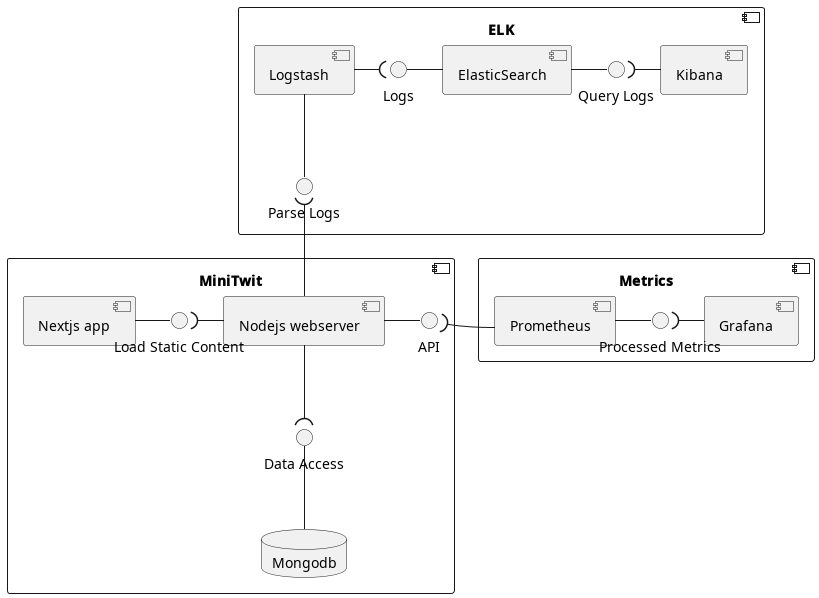
\includegraphics[scale=0.50]{component_diagram.png}
    \caption{Component Diagram}
    \label{componentdiagram}
\end{figure}

\subsection{Architecture of systems}

Since we chose to self-host our MiniTwit application, the full system architecture consists of a DELL PowerEdge R620, a NETGEAR GS748T managed switch, a 48 port LexCom patch panel and a custom 1U Supermicro box running OPNSense. 

\begin{figure}[H]
    \centering
    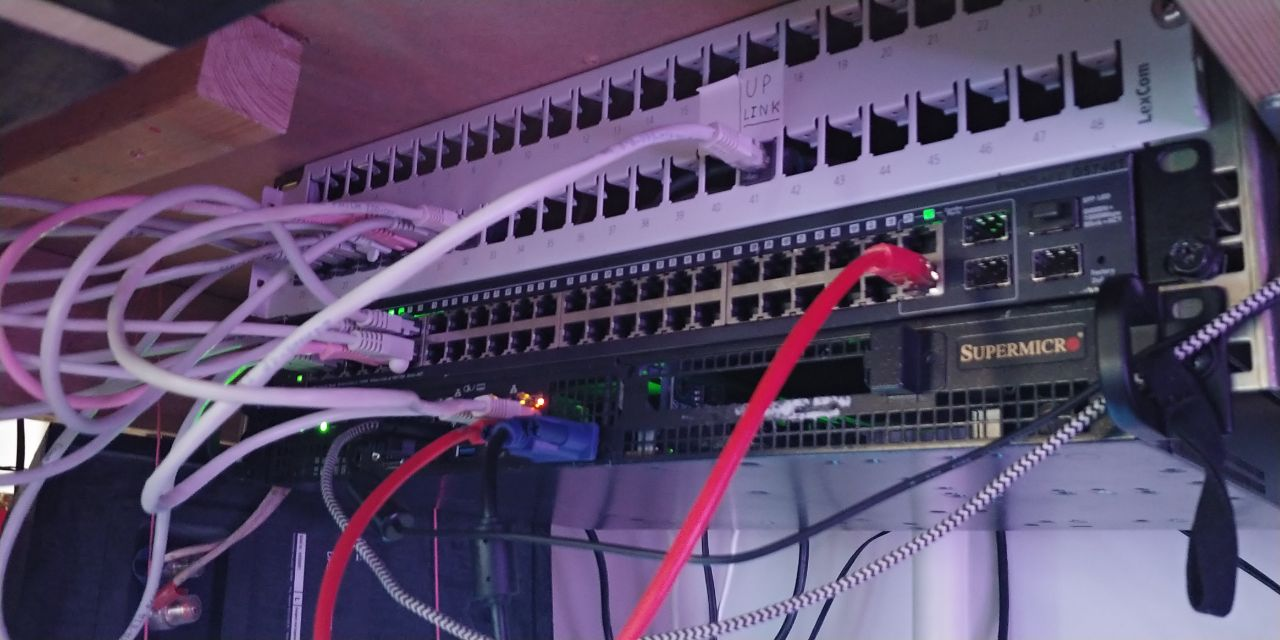
\includegraphics[scale=0.2]{network.jpg}
    \caption{A picture showing the network stack (from the top): LexCom patch panel, NETGEAR GS748T,  Supermicro box running OPNSense}
    \label{state}
\end{figure}

We are able to tag packets on different VLANs and separate traffic between the home and production network. Separating traffic provides better security and flexibility as it prevents packet sniffing from a possibly compromised host.

\begin{figure}[H]
    \centering
    \centerline{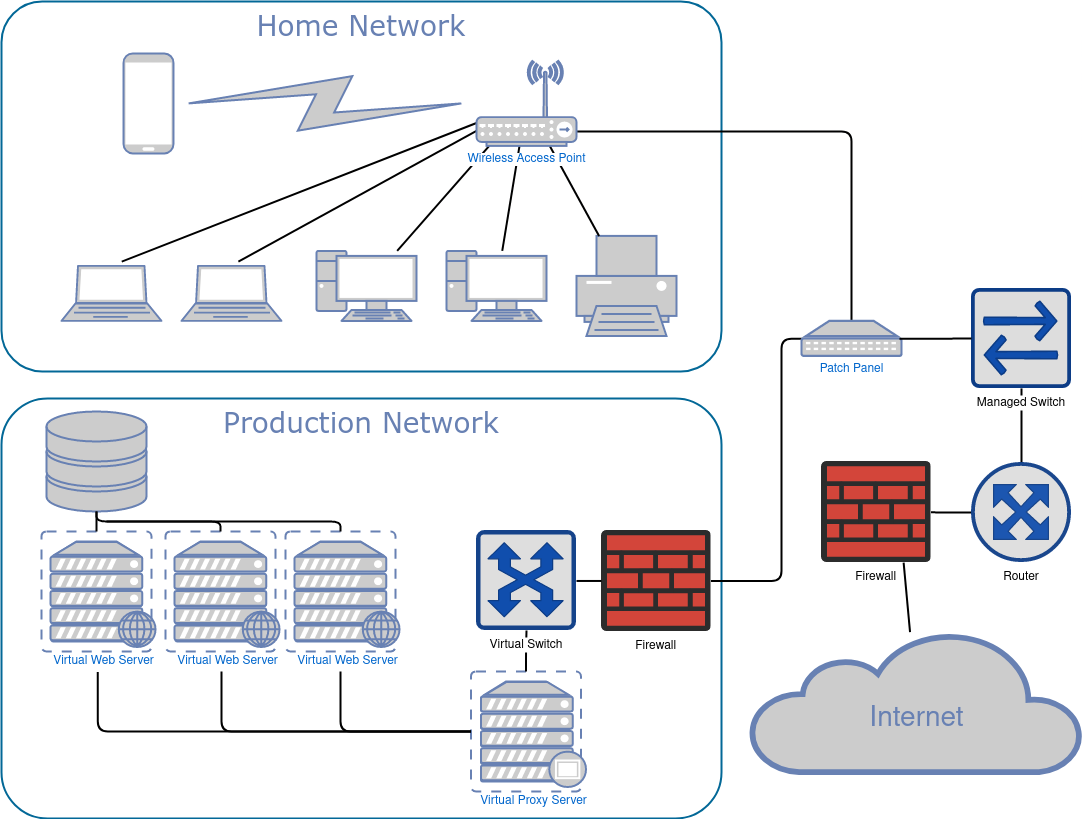
\includegraphics[scale=0.32]{WayNetwork.png}}
    \caption{A network diagram describing the setup of the WAY Network}
\end{figure}

Diving deeper into the subsystems, the MiniTwit app is specifically deployed on docker swarm, next to our various monitoring and logging services. All of this is on a virtual machine running Ubuntu 20.04.4 LTS, which itself is run on Proxmox \cite{proxmox}, a Type-1 hypervisor. Since Proxmox uses the Linux distribution "Debian" as its OS/kernel, KVM (Kernel-based Virtual Machine)\cite{kvm} is what allows for virtualization on the server. Most of the other web services on the server are run inside LXCs (Linux Containers) \cite{lxc}, but due to security concerns we decided to run the application inside a fully virtualized OS. 

\begin{figure}[H]
    \centering
    \centerline{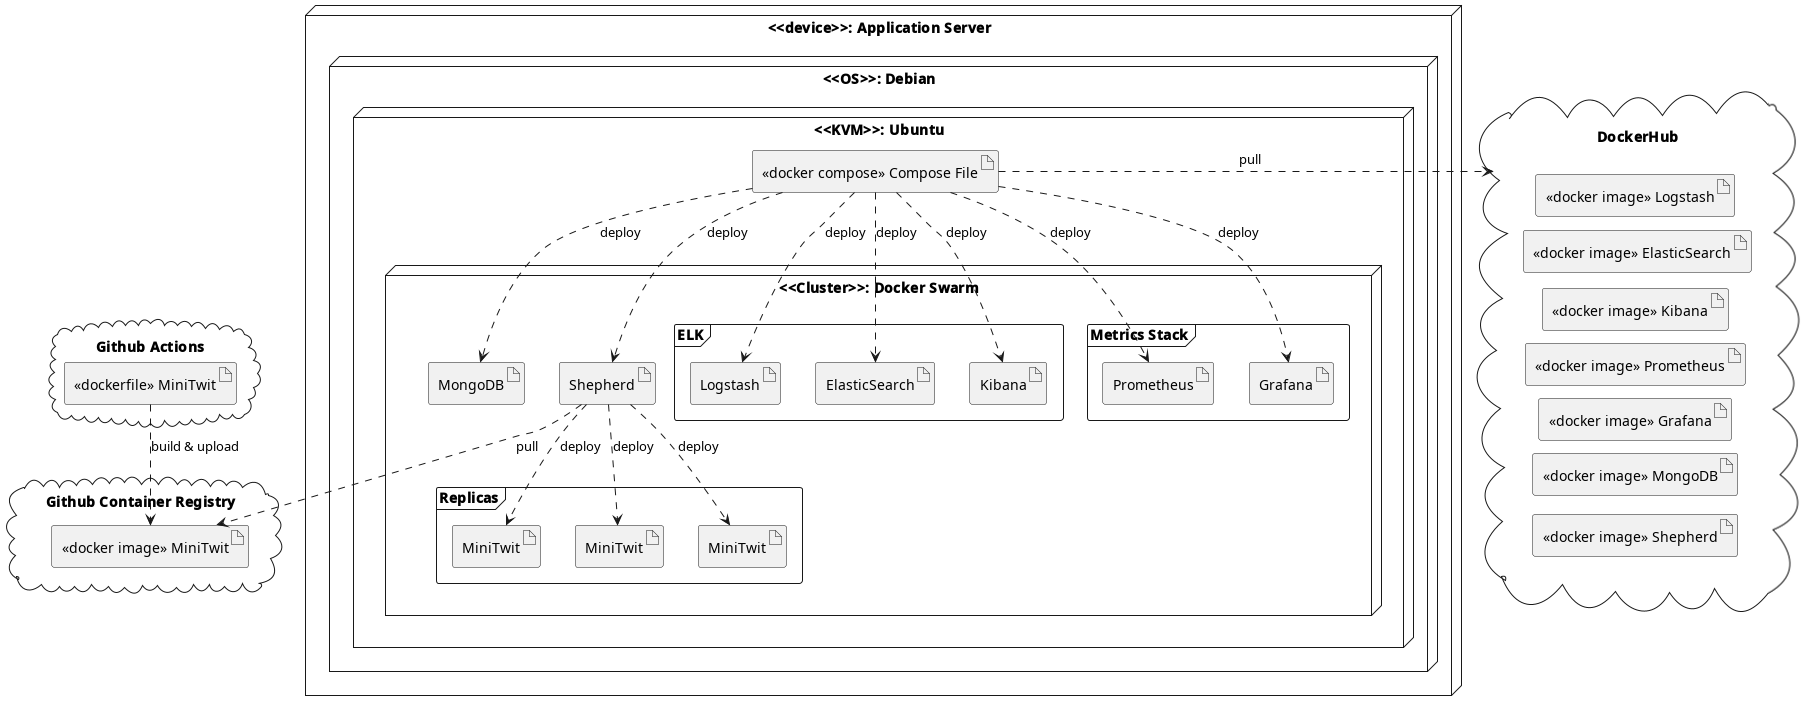
\includegraphics[scale=0.3]{deploy_diagram.png}}
    \caption{A diagram showing the deployment of our system}
\end{figure}

\subsection{Technologies and dependencies}
    
\textbf{Technologies:}
\begin{center}
\begin{tabularx}{0.8\textwidth} { 
  | >{\centering\arraybackslash}X 
  | >{\centering\arraybackslash}X 
  | >{\centering\arraybackslash}X |  }
 \hline
 Docker & Docker-Compose & Docker-swarm \\
 \hline
 Shepherd:latest  & Grafana:latest  & Prometheus:latest  \\
\hline
 ElasticSearch@8.1.1  & Kibana@8.1.1  & logstash@8.1.1  \\
\hline
 Mongo@4.4.12  &   &   \\
\hline
\end{tabularx}\\
\end{center}
\newpage
\textbf{Dependencies:}\\
The dependencies shown below is the top layer of the dependency graph.
\begin{center}
\begin{tabularx}{0.8\textwidth} { 
  | >{\centering\arraybackslash}X 
  | >{\centering\arraybackslash}X 
  | >{\centering\arraybackslash}X | }
 \hline
 aria-query@5.0.0 & axios@0.26.1 & bcryptjs@2.4.3 \\
 \hline
 classnames@2.3.1  & jsonwebtoken@8.5.1  & mongoose@6.3.0  \\
\hline
 next@12.1.5  & pino-caller@3.2.0  & pino-socket@4.1.1  \\
\hline
 pino@7.10.0  & prom-client@14.0.1  & react-dom@17.0.2  \\
\hline
 react@17.0.2  & sass@1.50.1  & sharp@0.30.4  \\
\hline
 stylelint-config-standard-scss@3.0.0  & 
 stylelint-config-standard@25.0.0  & stylelint@14.7.1  \\
\hline
 swr@1.3.0  & url-parse@1.5.10  &   \\
\hline
\end{tabularx}\\
\end{center}


\textbf {Tools:}\\
The table below contains all the tools we have used.
\begin{center}
\begin{tabularx}{0.8\textwidth} { 
  | >{\centering\arraybackslash}X 
  | >{\centering\arraybackslash}X 
  | >{\centering\arraybackslash}X | }
 \hline
 Docker (for development and deployment) & Dependabot (for packages) & 
  Nodejs (for source code) \\  
  \hline
 Snyk (for vulnerabilities)  &  Scancode (for license)  &  stylelint (for css styling)\\
\hline
 Sonarcloud.io  & LightHouse & CodeCov\\
\hline
\end{tabularx}
\end{center}


\subsection{Important interactions of subsystems}
% - Important interactions of subsystems
    % - What could the subsystems be? Find out more.
    % - Maybe Kibana, ElasticSearch, Grafana and so on?
    
We are using a variety of subsystems to make maintainability, identifying issues and monitoring easier.
\subsubsection{Prometheus Grafana Interaction} 
Prometheus is a tool used to monitor the performance of the system at run-time. In order for this data to be collected and displayed, we created a \textit{/metrics} API endpoint which contains all the collected data metrics.

Prometheus will periodically visit this endpoint, and collect and store the data. Grafana will connect to the Prometheus server, where it will hook into the data collected and display it on a dashboard.

\subsubsection{ELK Stack Interaction}
\label{ELK Stack Interaction}
The ELK stack consists of Logstash, ElasticSearch and Kibana. The purpose of the ELK stack is to track and visualize logs from the application. The type of logs are not related to performance like Prometheus, but related to how users interact with the application.

The ELK stack works by the application sending logs to a running Logstash server. Logstash parses the logs and ElasticSearch picks the parsed logs up. ElasticSearch adds functionality to search, sort, filter and more on the parsed logs from LogStash. In the end Kibana will connect with ElasticSearch and visualize all the logs in a clean and effective way.

A small detail about the way our application connects with the ELK-stack is by using a logging library called Pino. Pino observes all the incoming requests to the server and sends them to port 5000, where Logstash is listening. 


Refer to the \nameref{componentdiagram} that describes the above ELK interaction. Pino is a part of the Nodejs webserver in the diagram.

\subsection{Current state of system}
To objectively validate and test the current state of our system, we will use the three tools below for quality assessment.
\begin{itemize}
    \item Code analysis using Sonarcloud.io
    \item Test coverage and analysis using CodeCov
    \item Performance and accessibility testing using Lighthouse
\end{itemize}

\subsubsection{Code analysis}
We used Sonarcloud.io to make a static analysis report on our roughly 2500 lines of code. The result can be seen below.
\begin{figure}[H]
    \centering
    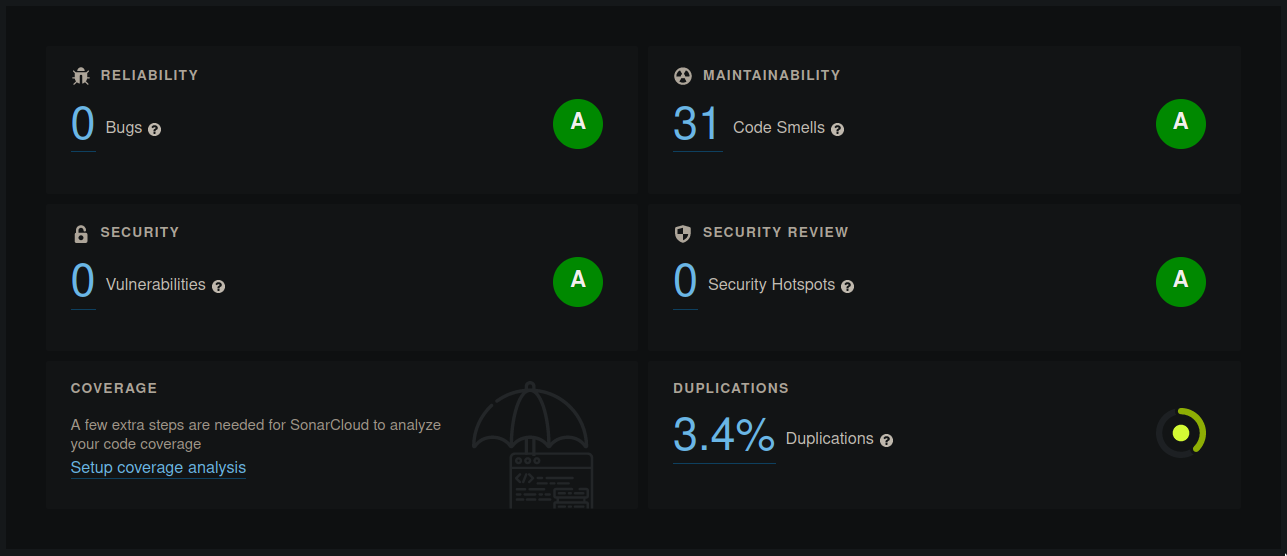
\includegraphics[scale=0.30]{images/sonarcloud.png}
    \caption{Static anlysis report from Sonarcloud.io}
\end{figure}

The result indicates that our code has 0 bugs, 0 security vulnerabilities, 0 security hotspots and 31 code smells. This does not guarantee that our code is bug-free or vulnerability-free, but is a great way of getting a general overview over the state of your code.
Furthermore, the report indicates that we have 3.4\% code duplication, meaning that the code is well structured with many reusable pieces of code. 

\subsubsection{Test coverage and analysis}
We made a test coverage report using CodeCov \cite{codecov}. The result can be seen below.
\begin{figure}[H]
    \centering
    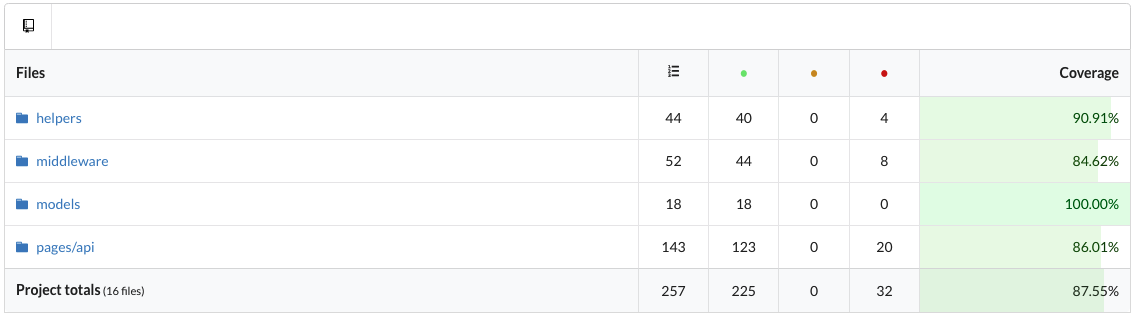
\includegraphics[scale=0.30]{images/codecov.png}
    \caption{Test coverage analysis from CodeCov}
\end{figure}

The result indicates that our code has an overall test coverage of 87.55\%. This is fairly high, indicating that most of the functionality has been tested thoroughly, to ensure little to no unexpected behaviour. 

\subsubsection{Performance and accessibility}
We made a performance and accessibility report using the Chromium tool, Lighthouse \cite{lighthouse}. The result of the report can be seen below.
\begin{figure}[H]
    \centering
    
\includegraphics[scale=0.50]{images/lighthouse.png}
    \caption{Performance and accessibility report from Lighthouse}
\end{figure}

The results of the report are divided into four sections; Performance, Accessibility, Best Practices and SEO.\\

The results above indicate that the application is in a satisfactory state according to Lighthouse's metrics. The application is performant and accessible as well as using favourable practices. 

\subsubsection{Conclusion}
When combining the results of the three reports, we can conclude that the current state of the system is of high quality and stable. The code is well written and bug free according to Sonarcloud.io, the code is well tested according to CodeCov and the application has satisfactory performance and accessibility.\\

The use of the three tools; Sonarcloud.io, CodeCov and Lighthouse helped us develop a better application and led to a better project overall.

\subsection{License of project}

The project is under the GPLv3 license\cite{gplv3}, because we want a very permissive license to make the project widely accessible to everyone and support copyleft licensing.

The GPLv3 license is compatible with the licenses of the dependencies we have used. We have carefully scanned our dependencies, to find that they either use MIT or Apache 2.0. These two types of licenses are compatible with GPLv3, and our project can therefore safely use all our dependencies.
\section{Process Perspective}

\subsection{Developer Interaction}
Throughout the entirety of this project, our interactions occurred through the following:
\begin{itemize}
    \item Weekly meetings, held both in-person at ITU and online
    \item Our Discord server
    \item Pair programming
    \item Issues and pull requests through GitHub
    \item Social gatherings outside the project
\end{itemize}

\subsection{Team Organization}
\subsubsection{Weekly Meetings}
At the end of every lecture, the group met and discussed the plan for the rest of the week, and gave a quick summary of the week prior, to ensure that everyone was on the same page. During weeks with high-workload, meetings would sometimes be scheduled for a later day, so the remaining work could be finished, and a release could be made.

\subsubsection{Separation of Work}
Throughout the project, we played to each other's strengths, while creating a learning environment that everyone benefited from. We primarily achieved this by making use of pair-programming, where we would pair someone experienced, on the specific technology, with someone inexperienced. This had very positive benefits, as the inexperienced person would always have someone to rely on, if they were to get stuck.

\subsection{CI/CD Chains}
\subsubsection{Continuous Integration (CI)}
All of our continuous integration chains are performed using GitHub Actions workflows. These workflows run based on different criteria.

\vspace{10pt}
\noindent
\textbf{Node.js} \textit{(node.js.yml)}\\
This workflow will automatically run on a push or pull configuration to the main branch. The workflow is responsible for making sure the application can build, as well as making sure that all tests pass. Furthermore, the workflow will upload the test results to CodeCov.

\vspace{10pt}
\noindent
\textbf{License scan} \textit{(scancode-toolkit.yml)}\\
This workflow will automatically run on a push or pull configuration to the main branch or every day at 12 PM via a cron job. This workflow is responsible for scanning the project for conflicting licenses from the dependencies we have used.

\vspace{10pt}
\noindent
\textbf{Vulnerabilities scan} \textit{(snyk-container.yml)}\\
This workflow will automatically run on a push or pull configuration from the main branch, or every Monday at 12 PM via a cron job. This workflow is responsible for scanning our Docker image for any vulnerabilities. This is done via a security tool from Snyk \cite{snyk}.\\

Any vulnerabilities found is uploaded to GitHub Code Scanning.

\vspace{10pt}
\noindent
\textbf{Styling and formatting scan} \textit{(stylelint.yml)}\\
This workflow will automatically run on a push or pull configuration to the main branch. This workflow is responsible for scanning our source code for any formatting or styling errors according to our set conventions. This is handled using Stylelint.

    
\subsubsection{Continuous Delivery (CD)}
In order to deploy a new version of the application to the production server, a new release must be published on GitHub which will trigger a GitHub Action workflow \textit{(docker-image.yml)} that will build a new Docker-image and push it to GitHub's container registry \textit{(ghcr.io)}.

Our production server will automatically pick up the new image by using a tool called Shepherd.\\

\noindent
\textbf{Shepherd}\\
Shepherd is a tool for automating the process of updating and redeploying docker containers running in a Docker Swarm Cluster. Shepherd itself runs in the Docker Swarm cluster on the production server and checks for new versions of other services in the cluster repeatedly at an interval of 5 minutes. When Shepherd finds a new version of an image it will download it and redeploy the corresponding container.\\

We are only using this approach for the \textit{MiniTwit} service in the cluster, because pulling repeatedly from Docker Hub (where our other images are hosted) would get us rate limited for pulling too many times and therefore not being able to update the images.

    
\subsection{Repository Organization}
The repository of our application is a mono-repository including both the front-end and the back-end. The back-end part of the application is closely integrated with the front-end.\\

Furthermore, the clean file structure that Next.js has to offer makes mono-repositories easy and efficient to manage for applications at this size.

% - Applied branching strategy. - Deniz Y
\subsection{Applied Branching Strategy}
In the beginning of the project, we created a \href{https://github.com/AlexBMJ/minitwit/blob/main/CONTRIBUTING.md}{CONTRIBUTING.md} file for everyone to follow. This file includes a description of our branching strategy, git workflow, responsibility of each member, etc. 

\subsection{Applied Development Process \& Tools Supporting It}
Throughout the course, we primarily used the Software Development cycle process \cite{sdc}. This process consists of 6 steps, and is an iterative process:
\begin{figure}[H]
    \centering
    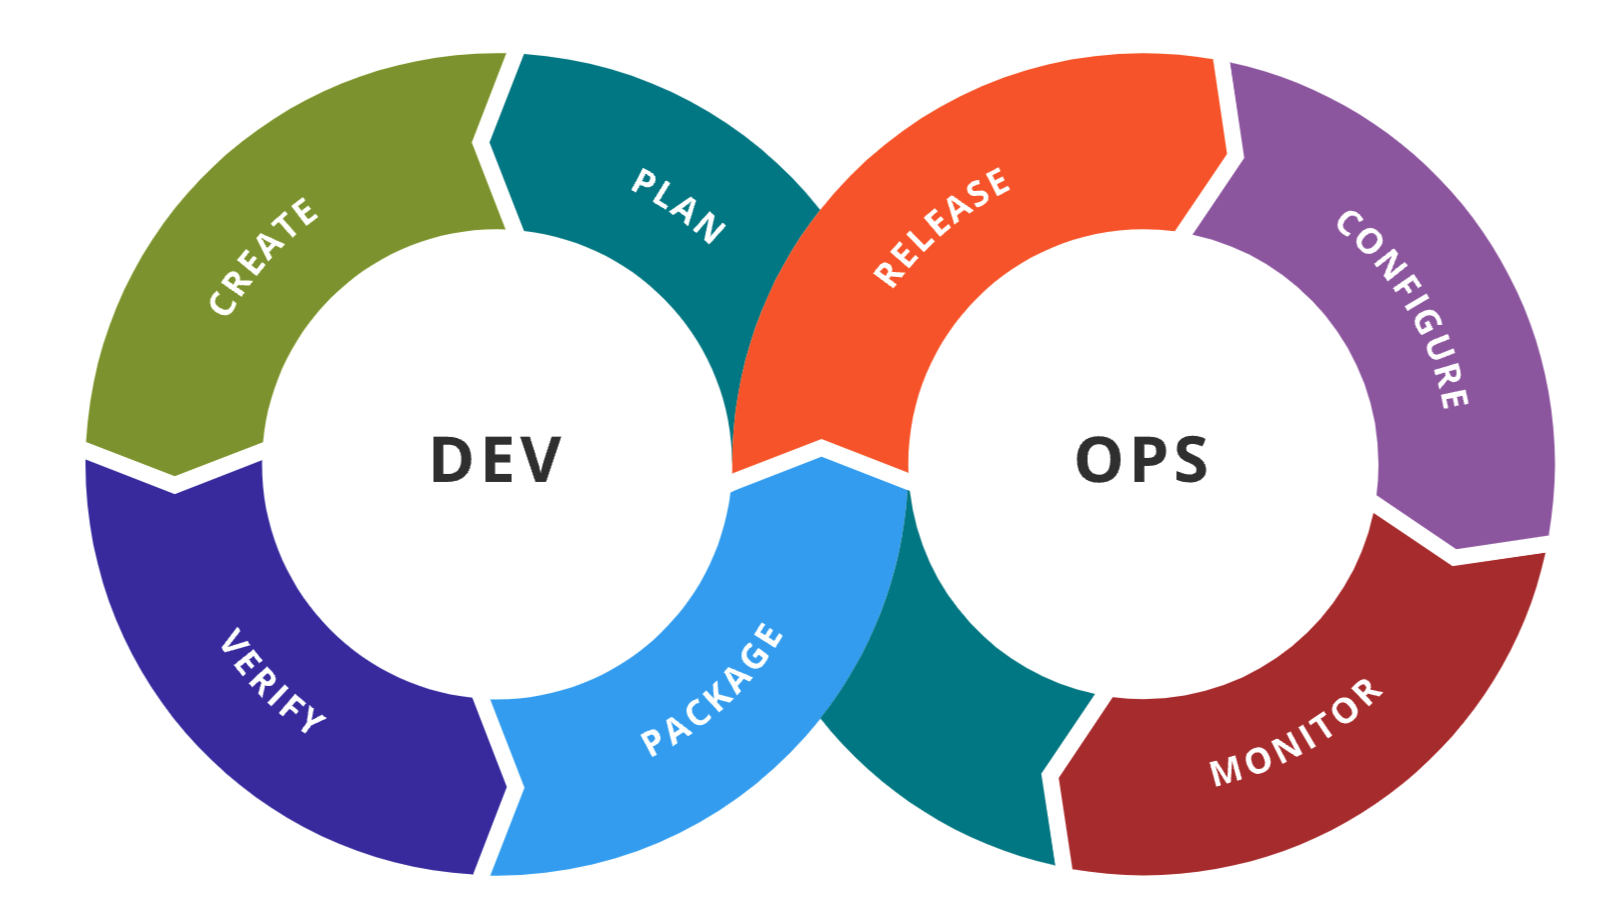
\includegraphics[scale=0.20]{images/sdc.png}
    \caption{Software Development Cycle}
\end{figure}
When there were parts of the project that we did not manage to complete in time, or found bugs that we did not have enough time to fix, we would create an issue on GitHub, and schedule a time to meet throughout the week to fix those issues. This was an excellent way to plan ahead.

Besides GitHub issues, we did not use any development tools to assist us. This was because the course was structured in such a way, in which we already were aware of what needed to be done each week.

\subsection{Monitoring}
\begin{enumerate}
    \item  Monitoring on Kibana (logging)
    \item  Monitoring on Grafana (server side)
\end{enumerate}
We are using Grafana and Kibana to monitor our application. Grafana is mainly used to monitor the applications performance metrics and Kibana is used to monitor logging. 
We are using Prometheus which is a metrics parser that stores information that changes over time.\\

The importance of Grafana is mainly to give us a visual overview of the different parts of the system and alert us if something is wrong, for instance if the system goes down. We are using a webhook to send the alerts into our Discord server, but we do also have mail notifications enabled if the Discord webhook fails. That way can quickly and efficiently fix occurring issues.

\begin{figure}[H]
    \centering
    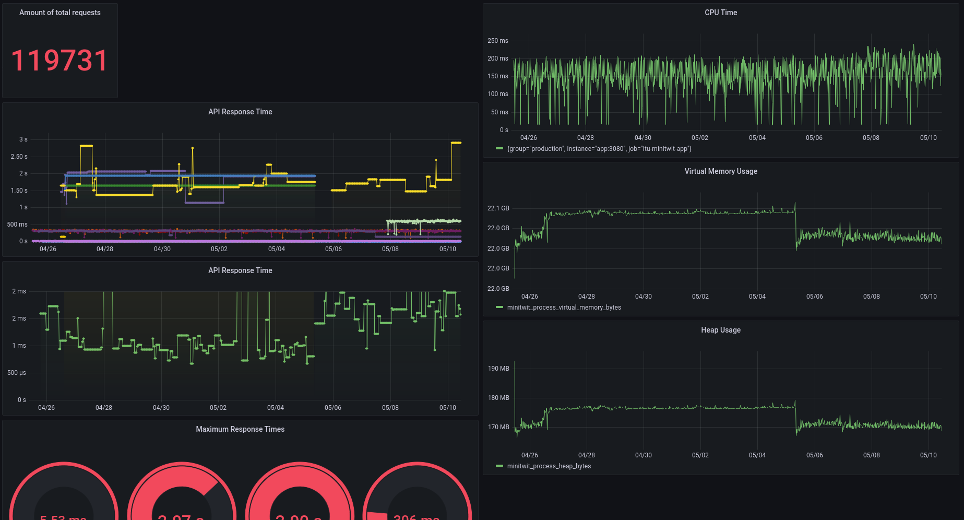
\includegraphics[scale=0.8]{images/Grafana.png}
    \caption{Grafana graphical representation of the application and its server}
\end{figure}

\begin{figure}[H]
    \centering
    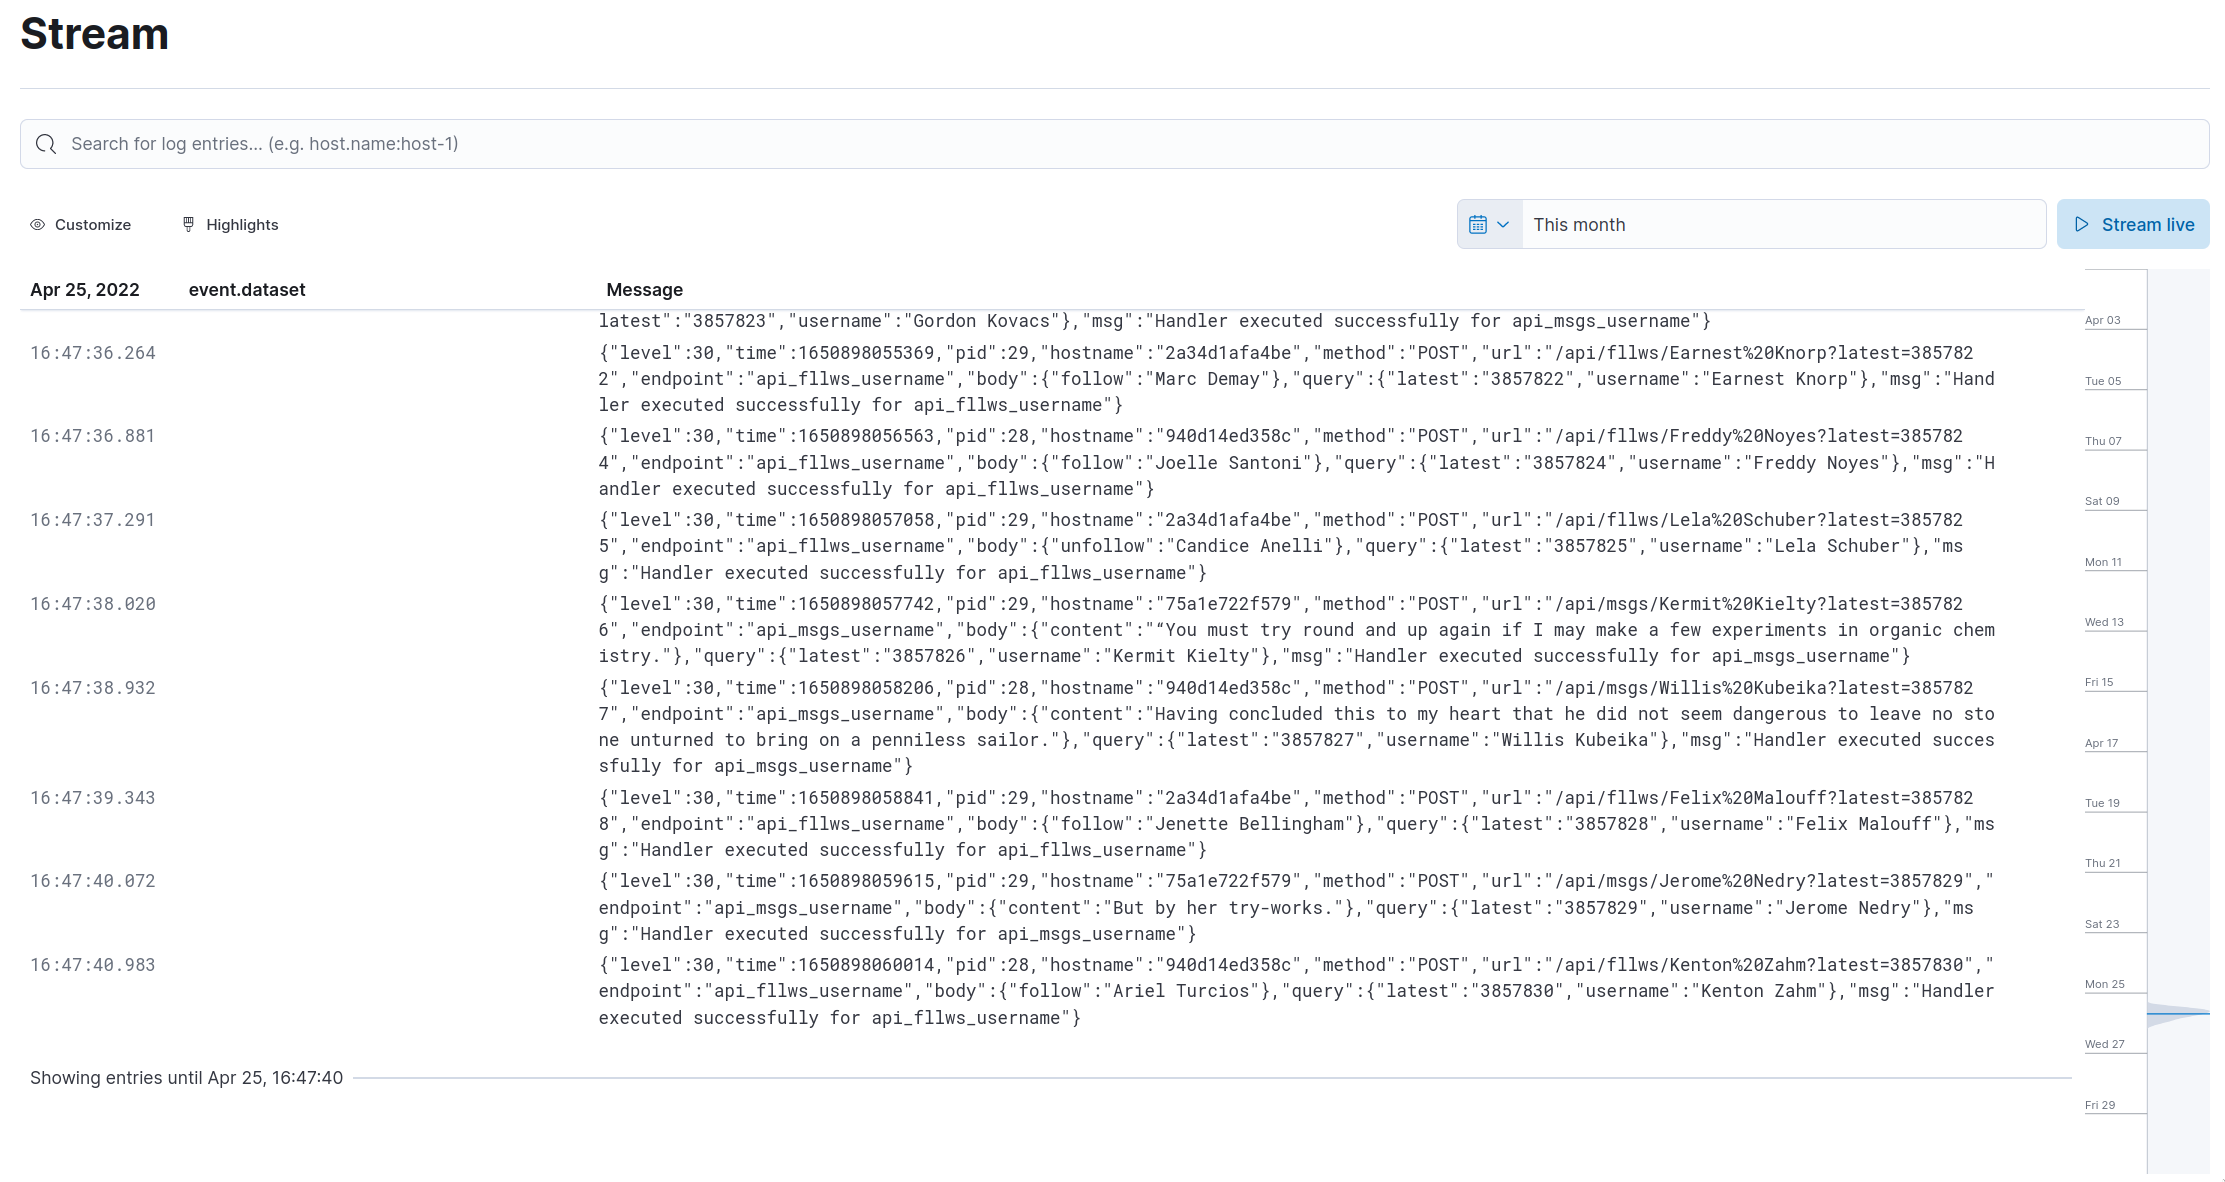
\includegraphics[scale=0.2]{images/kibana.png}
    \caption{Kibana dashboard showing logs}
\end{figure}


\subsection{Logging \& Aggregation}
% - What do you log in your systems and how do you aggregate logs? - Deniz I
We are using the library Pino to create Syslog entries for all our API endpoints by having the requests go through our \textit{MiniTwitRoute} middleware.
The log entries include the query method, url, endpoint, body, and query of the HTTP requests.
All of the logs are then aggregated to ElasticSearch as explained in section \ref{ELK Stack Interaction}, where we can easily search and filter through them.

Some of the API endpoints include those used for sending messages, following users, and signing in.

It is worth noting that ElasticSearch unfortunately only shows logs for the first few hours of the application start due to an unresolved bug. We narrowed down the issue to be related to Pino, but sadly could not investigate further as the course came to an end.

\subsection{Security Assessment Results}
% - Brief results of the security assessment. - Deniz I

\begin{figure}[H]

\begin{center}
    \begin{tabular}{ |c|p{12em}|c|c|c|c| } 
        \hline
        & Rare & Unlikely & Possible & Likely & Certain \\
        \hline
        Catastrophic & SQL injection / MITM  \cellcolor{orange} & \cellcolor{orange} &  \cellcolor{red} &  \cellcolor{red} & \cellcolor{red} \\ 
        \hline
        Critical &  Automatic re-deployment \cellcolor{orange} & DDOS \cellcolor{orange} &  \cellcolor{orange} & \cellcolor{red} &  \cellcolor{red}\\ 
        \hline
        Marginal &  \cellcolor{green} & \cellcolor{orange}  &  \cellcolor{orange} &  \cellcolor{orange} &  \cellcolor{red} \\ 
        \hline
        Negligible &  \cellcolor{green} & \cellcolor{green}   &  \cellcolor{orange} &  \cellcolor{orange} &   \cellcolor{orange} \\ 
        \hline
        Insignificant & \cellcolor{green} \cellcolor{green} & \cellcolor{green} &  Prometheus metrics \cellcolor{green} &  \cellcolor{orange} &  \cellcolor{orange} \\
        \hline
    \end{tabular}
\end{center}
    \centering
    \caption{Risk assesment matrix}
\end{figure}

\subsubsection{Risk identification}
Our risk assessment matrix table shows 5 possible scenarios:

\textbf{SQL-injection:}
SQL-injections are in today's world a catch-all phrase for the injection of database query languages. Despite the use of a NoSQL database, possible vulnerabilities which allow an attacker to manipulate or retrieve data, could still be possible. 
\vspace{10pt}
\noindent

\textbf{MITM:}
In the beginning we did not have a TLS certificate for the website which could have resulted in a "man in the middle"-attack. Without a TLS certificate data is being transferred from client to server in clear text without encryption. However, we discovered the threat source quickly and mitigated it by installing a TLS certificate.

\vspace{10pt}
\noindent
\textbf{Automatic redeployment:}
If an attacker were to upload an image to the container repository Shepard is pulling from, it would result in potentially malicious code being run on the production server.

\vspace{10pt}
\noindent
\textbf{Prometheus metrics:}
The Prometheus npm package exposes a metrics page with various statistics and is the data displayed in Grafana. This page is technically only needed by Prometheus running on the same host, but is also reachable from the outside world. 

\vspace{10pt}
\noindent
\textbf{DDOS:}
Since we are hosting the server in a residential building and not in a datacenter, we have no dedicated protection against "Distributed denial of service" (DDOS) attacks \cite{ddos}. A DDOS attack would therefore leave our application unresponsive.

\subsubsection{Risk analysis}

\textbf{SQL-injection:} We rate the likelihood of a SQL-injection occurring to be low since we use an ODM-library (Object Document Mapping) and therefore not sending raw queries to the database.\\

\textbf{MITM:} We rate the likelihood of a "man in the middle"-attack occurring to be low since we now use a TLS certificate.\\

\textbf{Automatic redeployment:} We rate the likelihood of a malicious image being pushed into our GitHub Package Registry to be low since it requires access to an authorized GitHub account.\\

\textbf{Exposing Prometheus metrics:} We rate the likelihood of finding the Prometheus endpoint to be medium since it is public, but is not indexed or listed. This means an attacker would have to use a bruteforce crawler to discover the path.\\

\textbf{DDOS:} We rate the likelihood of a DDOS-attack occurring to be very low, since our application is not very popular nor does the attacker have anything to gain by making our small course project unresponsive.\\

\subsection{Scaling and Load Balancing}
Both scaling and load balancing of our application is managed automatically by Docker Swarm. We have not scaled our system horizontally, but if we were to do so, it would be easy as Docker Swarm uses the Raft consensus algorithm\cite{raft}. The system is scaled vertically once because we wanted to have three replicas of our application running in the cluster. For load balancing, Docker Swarm uses ingress load balancing which is an object that manages external access to the cluster's services and automatically distributes traffic across the replicas through a shared access point.

\newpage
\section{Lessons Learned Perspective}
\subsection{Evolution and refactoring}
\subsubsection{Refactoring}
Throughout the project, we learned the importance of continuously refactoring the application to use the latest and best practices. Doing so brings performance improvements, makes the code easier to maintain and extend as well as overall security posture.

We have learned that while refactoring is a good practice, it can often not be done in parts if the application is tightly connected. Therefore, refactoring often impacts many parts of the application and requires a lot of work. An example of this can be found in our refactor from \href{https://github.com/AlexBMJ/minitwit/pull/2}{pull request \#2}. 

As noted before, we were continuously refactoring aspects of our program that we were not happy with, or thought could be better. This was an iterative process that lasted the entirety of the project. An example of this is our \href{https://github.com/AlexBMJ/minitwit/pull/35}{35th pull request}.

\subsubsection{Evolution}
Once the application became ready for deployment, we put a high priority on automating as much as we could. In the beginning, we had to manually deploy the application, and that quickly became an apparent obstacle that had to get solved using continuous deployment. Our main takeaway is that it was valuable to have automation from the beginning. It is apparent that minimizing manual work, allows for time spent on development instead of deployment.
Moving forward, we will continue to prioritize automation in all aspects of DevOps life-cycle.

We realized how motivational graphs and statistics can be, but more importantly it allows for a better insight into our application and how to improve it. Once we had set up Grafana, we could easily see how well our application was doing and in what areas. Moving forward, setting up performance monitoring is something we want to add as it is an important part of discovering performance issues and obscure bugs.

\subsection{Operation}
When merging to and setting up the production environment, we ran into an issue regarding the hardware of our self-hosted server. The version of MongoDB that we had been using in local development, was not supported by the CPU architecture that our self-hosted server ran on. 

This resulted in us having to downgrade our MongoDB database to version 4.4. This is not optimal for the operation of the application, but was a necessity with our setup. The downgrade can be seen in \href{https://github.com/AlexBMJ/minitwit/pull/10}{pull request \#10}.

This lesson taught us that the physical hardware is just as important to update as the software dependencies which runs upon it. Especially, if you want to maintain a secure and stable version of your application.

\subsection{Maintenance}
In order to make parts of maintaining our application autonomous, we used tools such as \textbf{Dependabot} and \textbf{Snyk}.

\subsubsection{Dependabot}
Dependabot helps us ensure that the dependencies we use are always up to date, so when a new update is released, a pull request is made with the update. This ended up helping us immensely, as library updates were continuously released throughout the life-span of the project. This ensured that we had the latest bug fixes and security updates.

An example of how effective Dependabot is, can be seen in our current open pull requests:
\begin{figure}[H]
    \centering
    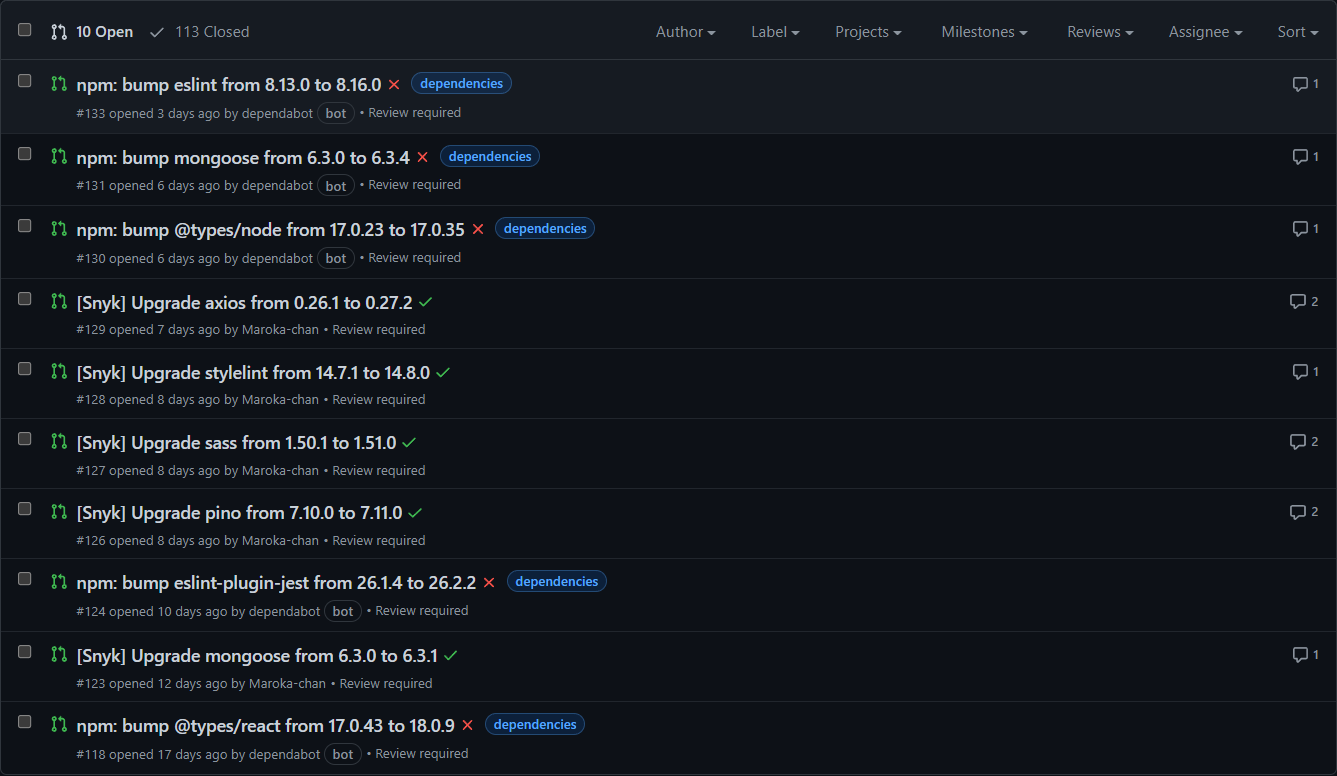
\includegraphics[scale=0.45]{images/dependabot.png}
    \caption{Dependabot notifying us about new dependency versions }
\end{figure}

\newpage
\subsubsection{Snyk}
Snyk looks at our docker image to find vulnerabilities and notifies us if any are found.

An example of Snyk scanning for vulnerabilities can be found \href{https://github.com/AlexBMJ/minitwit/runs/6539384679?check_suite_focus=true}{here}, where Snyk reported \textit{``Tested 17 dependencies for known issues, no vulnerable paths found``}.

An example of the repository's security tab, which is what Snyk reports to, can be found here:
\begin{figure}[H]
    \centering
    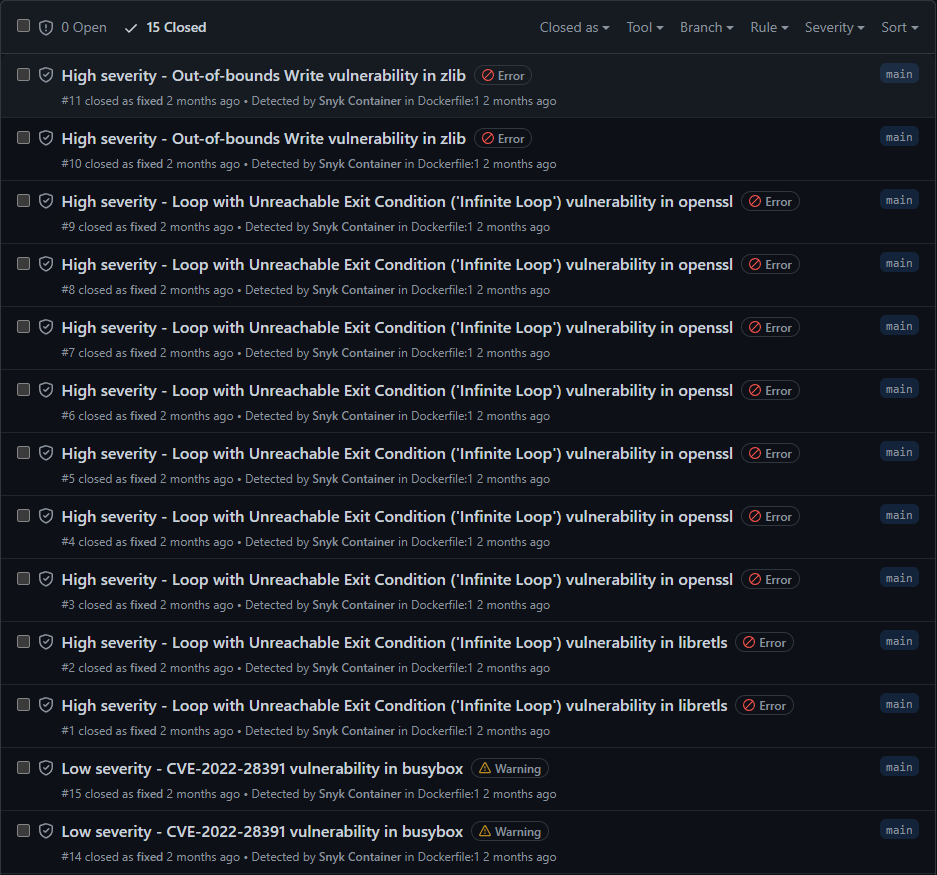
\includegraphics[scale=0.40]{images/snyk.png}
    \caption{Snyk found potential vulnerabilities}
\end{figure}

\paragraph{Lessons Learned}
These tools taught us how easy it is to maintain dependencies and minimize the threat surface of our application. We have been made considerably more aware of how important it is to continuously monitor vulnerabilities and maintain the system as a whole, including source code, packages and deployment.

\section{Conclusion}
Throughout the project, we took a legacy version of the MiniTwit application and refactored it into a modern maintainable TypeScript application. We took advantage of a multitude of DevOps principles to enhance the application, using several tools and techniques. This has benefited the overall application in many ways, as documented throughout this report. It has become abundantly clear to us how important it is to work with a DevOps mindset, and to use those principles for future projects when given the chance.

\newpage
\section{References}
\printbibliography[heading=none]

\end{document}
